\section{Methods}

\subsection{Nearest neighbor interpolation}
In nearest neighbor interpolation, we process the raw Bayer data in squares of
4 pixels, which contain 1 red, 1 blue and 2 green pixels. For the blue
channel, all 4 pixels are set to the color value of the 1 blue pixel. The same
is done for the red channel. For the green channel, the pixels without a green
color value get their value from the green pixel horizontally next to them.

The main benefits of NN-interpolation are its speed and simplicity.

\subsection{Bilinear interpolation}

In bilinear interpolation the color value of the pixels is calculated from the
color value of neighboring pixels with same color i.e sum the values of
neighboring pixels and divide it by the amount of neighboring pixels. However,
the pixels at the edges of the picture don't always have neighboring pixels
with color value or don't have enough of them. To correct this we can just
ignore the border pixels, resulting in smaller image, or as we did in the
assignment and pad the color arrays with zeros. The color values of the layers
are in different pixels, so every layer needs an unique function to calculate
the value of an unknown pixel.  Green has the most known color values, and
every unknown pixel borders four known pixels, so one function can calculate
all values of the green layer.

Only every other row of red and green layers has colorvalues, which has to be
taken into account when designing these functions. The rows which have no
colorvalues compute the value differently, depending on how many known values
border the pixel, and use either four or two values.

Colorvalues of the pixels are calculated from the padded color array and added
to the unpadded one. After all values of all colorarrays are calculated, the
arrays are combined into RGB image.

\subsection{Patterned pixel grouping interpolation}
The Patterned Pixel Grouping, or PPG interpolation is a significantly more
advanced method of interpolation. We implemented the method using the
description found here\cite{chuan-kai_lin}.

This method basically tries to take into account the color gradients found in
the data. It also takes advantage of the greater amount of green data and uses
it to assess the brightness gradients of the image, which is a feature that the
human visual system perceives more accurately than changes in color.
Figure~\ref{fig:bayer-pattern} has an example of Bayer data, which we'll refer
to when explaining the method.

\begin{figure}[H]
  \centering
  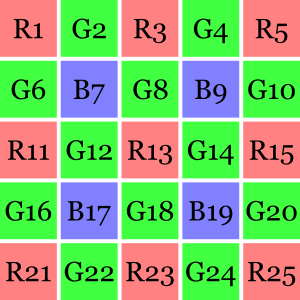
\includegraphics[width=0.8\linewidth]{bayer-pattern}
  \caption{The example portion of the data used in patterned pixel
    grouping~\cite{chuan-kai_lin}}
\label{fig:bayer-pattern}
\end{figure}


First the method calculates a value for all the missing green pixels. It
calculates the values by first assessing 4 gradients, in the cardinal
directions, using two neighboring green pixels and the red/blue pixel in place
of the missing green pixel and the red/blue pixel in the cardinal direction.
For example, the ``northern'' gradient for pixel 13 in~\ref{fig:bayer-pattern}
is calculated using formula~\ref{eq:nGradient}

\begin{equation}
  \label{eq:nGradient}
  \Delta N = | R_{13} - R_3 | \times 2 + | G_8 - G_{18} |
\end{equation}

The pixels used in the calculation of the smallest gradient are then used to
calculate the actual green color value for the pixel, as shown in
equation~\ref{eq:nValue}, which calculates the value in the case of the
northern gradient being smallest.

\begin{equation}
  \label{eq:nValue}
  G_{13} = (G_8 \times 3 + G_{18} + R_{13} −- R_3) / 4
\end{equation}

After the green values are calculated for every pixel, the missing red and blue
values are calculated. The instructions~\cite{chuan-kai_lin} use an auxiliary
function called \textit{hue\_transit}, defined as:

\begin{verbatim}
  function hue_transit (l1, l2, l3, v1, v3) =
    if (l1 < l2 and l2 < l3) or (l1 > l2 and l2 > l3)
    then v1 + (v3 − v1) × (l2 − l1) / (l3 − l1)
    else (v1 + v3) / 2 + (l2 × 2 − l1 − l3) / 4
\end{verbatim}

The red and blue pixels that are situated on top of only green pixels are
calculated using only this function. For example, the blue value of pixel 8 in
the data~\ref{fig:bayer-pattern} is calculated with equation~\ref{eq:blue8}

\begin{equation}
  \label{eq:blue8}
  B_8 = hue\_transit(G_7, G_8, G_9, B_7, B_9)
\end{equation}


For pixels where there's already a red or blue value, the method is a bit more
complicated. First, we again calculate gradients, this time however only two: A
north-east to south-west gradient and a north-west to south-east gradient. For
example, the NE to SE gradient for the blue value of pixel 13 is calculated
with formula~\ref{eq:neGradient}

\begin{equation}
  \label{eq:neGradient}
  \Delta NE = | B_9 −- B_{17} | + | R_5 −- R_{13} | + | R_{13} -− R_{21} | + | G_9
  −- G_{13} | + | G_{13} -− G_{17} |
\end{equation}

The gradients are then compared again, and for example if the \(\Delta NE\)
gradient is smaller, equation~\ref{eq:neValue} gives the blue value for pixel
13.

\begin{equation}
  \label{eq:neValue}
  B_{13} = hue\_transit(G_9, G_{13}, G_{17}, B_9, B_{17})
\end{equation}




















